\documentclass[fleqn]{article}\usepackage[]{graphicx}\usepackage[]{color}
% maxwidth is the original width if it is less than linewidth
% otherwise use linewidth (to make sure the graphics do not exceed the margin)
\makeatletter
\def\maxwidth{ %
  \ifdim\Gin@nat@width>\linewidth
    \linewidth
  \else
    \Gin@nat@width
  \fi
}
\makeatother

\definecolor{fgcolor}{rgb}{0.345, 0.345, 0.345}
\newcommand{\hlnum}[1]{\textcolor[rgb]{0.686,0.059,0.569}{#1}}%
\newcommand{\hlstr}[1]{\textcolor[rgb]{0.192,0.494,0.8}{#1}}%
\newcommand{\hlcom}[1]{\textcolor[rgb]{0.678,0.584,0.686}{\textit{#1}}}%
\newcommand{\hlopt}[1]{\textcolor[rgb]{0,0,0}{#1}}%
\newcommand{\hlstd}[1]{\textcolor[rgb]{0.345,0.345,0.345}{#1}}%
\newcommand{\hlkwa}[1]{\textcolor[rgb]{0.161,0.373,0.58}{\textbf{#1}}}%
\newcommand{\hlkwb}[1]{\textcolor[rgb]{0.69,0.353,0.396}{#1}}%
\newcommand{\hlkwc}[1]{\textcolor[rgb]{0.333,0.667,0.333}{#1}}%
\newcommand{\hlkwd}[1]{\textcolor[rgb]{0.737,0.353,0.396}{\textbf{#1}}}%
\let\hlipl\hlkwb

\usepackage{framed}
\makeatletter
\newenvironment{kframe}{%
 \def\at@end@of@kframe{}%
 \ifinner\ifhmode%
  \def\at@end@of@kframe{\end{minipage}}%
  \begin{minipage}{\columnwidth}%
 \fi\fi%
 \def\FrameCommand##1{\hskip\@totalleftmargin \hskip-\fboxsep
 \colorbox{shadecolor}{##1}\hskip-\fboxsep
     % There is no \\@totalrightmargin, so:
     \hskip-\linewidth \hskip-\@totalleftmargin \hskip\columnwidth}%
 \MakeFramed {\advance\hsize-\width
   \@totalleftmargin\z@ \linewidth\hsize
   \@setminipage}}%
 {\par\unskip\endMakeFramed%
 \at@end@of@kframe}
\makeatother

\definecolor{shadecolor}{rgb}{.97, .97, .97}
\definecolor{messagecolor}{rgb}{0, 0, 0}
\definecolor{warningcolor}{rgb}{1, 0, 1}
\definecolor{errorcolor}{rgb}{1, 0, 0}
\newenvironment{knitrout}{}{} % an empty environment to be redefined in TeX

\usepackage{alltt}
\usepackage{amsmath}
\usepackage{amssymb}
\usepackage{geometry}
\usepackage{graphicx}
\usepackage{bm}
\usepackage{url}
\usepackage{enumerate}
\usepackage{fullpage}
\IfFileExists{upquote.sty}{\usepackage{upquote}}{}
\begin{document}
\setlength\parindent{0pt}

\begin{center}
\large
\textbf{Lecture 5: Sampling Distributions and The Central Limit Theorem}\\
\normalsize
\textbf{STAT 630, Fall 2021}\\
\hrulefill
\end{center}

Recall that:
\begin{itemize}
\item A \textbf{parameter} is a numerical summary of a population (e.g., the population mean $\mu$).  It is a fixed number and usually unknown.
\item A \textbf{statistic} is a numerical summary of a sample (e.g., the sample mean $\bar{x}$).  It is random since it varies from sample to sample.\\
\end{itemize}

A \textbf{sampling distribution} is the distribution of values of a statistic when repeatedly taking random samples of the same size from a population.\\  


\textbf{Simulation Study}\\  
Suppose a population has a uniform distribution between 0 and 1, denoted by $U(0,1)$.  
\begin{enumerate}[(a)]
\item Let $X$ be a random variable such that $X \sim U(0,1)$.  Find the mean and variance of $X$?\\
\vspace{7cm}

% {\color{blue} 
% The probability density function for $X \sim U(0,1)$ is given by
% \begin{align*}
% f(x) =
% \begin{cases}
% 1, & 0 \leq x \leq 1\\
% 0, & \text{otherwise}
% \end{cases}
% \end{align*}
% 
% \begin{align*}
% \mu = E(X) = \int_0^1 x f(x) dx = \int_0^1 x dx = \frac{x^2}{2} \Big |_0^1 = \frac{1}{2}
% \end{align*}
% 
% To compute the variance use $Var(X) = E(X^2) - [E(X)]^2 = E(X^2) - \mu^2$
% \begin{align*}
% E(X^2) = \int_0^1 x^2 f(x) dx = \int_0^1 x^2 dx = \frac{x^3}{3} \Big |_0^1 = \frac{1}{3}
% \end{align*}
% Therefore,
% \begin{align*}
% \sigma^2 = Var(X) = E(X^2) - \mu^2 = \frac{1}{3} - \frac{1}{4} = \frac{1}{12}
% \end{align*}
% }

\clearpage
\item Use R to draw 1000 random numbers from $U(0,1)$.  Make a histogram and normal QQ plot of the values.  Also, compute the mean and variance of the values.
\begin{knitrout}
\definecolor{shadecolor}{rgb}{0.969, 0.969, 0.969}\color{fgcolor}\begin{kframe}
\begin{alltt}
\hlkwd{set.seed}\hlstd{(}\hlnum{100}\hlstd{)}
\hlstd{u} \hlkwb{<-} \hlkwd{runif}\hlstd{(}\hlnum{1000}\hlstd{)}

\hlkwd{par}\hlstd{(}\hlkwc{mfrow}\hlstd{=}\hlkwd{c}\hlstd{(}\hlnum{1}\hlstd{,}\hlnum{2}\hlstd{),} \hlkwc{cex}\hlstd{=}\hlnum{0.6}\hlstd{)}
\hlkwd{hist}\hlstd{(u)}
\hlkwd{qqnorm}\hlstd{(u)}
\hlkwd{qqline}\hlstd{(u)}
\end{alltt}
\end{kframe}
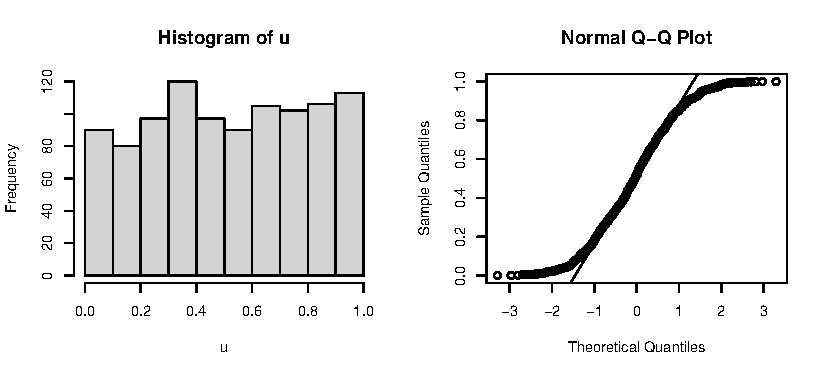
\includegraphics[width=\maxwidth]{figure/unnamed-chunk-1-1} 
\begin{kframe}\begin{alltt}
\hlkwd{mean}\hlstd{(u)}
\end{alltt}
\begin{verbatim}
## [1] 0.5180817
\end{verbatim}
\begin{alltt}
\hlkwd{var}\hlstd{(u)} \hlcom{# close to 1/12 = 0.0833}
\end{alltt}
\begin{verbatim}
## [1] 0.08254194
\end{verbatim}
\end{kframe}
\end{knitrout}
\bigskip

% {\color{blue}
% Notice that:
% \begin{align*}
% \texttt{mean(u)} &\approx 0.5 = E(X) = \mu\\
% \texttt{var(u)} &\approx \frac{1}{12} = Var(X) = \sigma^2
% \end{align*}
% }

\clearpage

\item Use R to repeatedly draw 1000 samples of size $n=2$ from $U(0,1)$.  Take the sample mean of the values in each sample.  Make a histogram and normal QQ plot of the 1000 sample means.  Compute the mean and variance of the sample means.  What do you notice? 
\begin{knitrout}
\definecolor{shadecolor}{rgb}{0.969, 0.969, 0.969}\color{fgcolor}\begin{kframe}
\begin{alltt}
\hlkwd{set.seed}\hlstd{(}\hlnum{100}\hlstd{)}
\hlstd{xbars} \hlkwb{<-} \hlkwd{rep}\hlstd{(}\hlnum{0}\hlstd{,} \hlnum{1000}\hlstd{)} \hlcom{# initialize vector }
\hlkwa{for}\hlstd{(i} \hlkwa{in} \hlnum{1}\hlopt{:}\hlnum{1000}\hlstd{) \{}
  \hlstd{samp} \hlkwb{<-} \hlkwd{runif}\hlstd{(}\hlnum{2}\hlstd{)}
  \hlstd{xbars[i]} \hlkwb{<-} \hlkwd{mean}\hlstd{(samp)}
\hlstd{\}}

\hlkwd{par}\hlstd{(}\hlkwc{mfrow}\hlstd{=}\hlkwd{c}\hlstd{(}\hlnum{1}\hlstd{,}\hlnum{2}\hlstd{),} \hlkwc{cex}\hlstd{=}\hlnum{0.6}\hlstd{)}
\hlkwd{hist}\hlstd{(xbars,} \hlkwc{main} \hlstd{=} \hlstr{"Histogram of sample means (n=2)"}\hlstd{,} \hlkwc{xlab}\hlstd{=}\hlstr{''}\hlstd{)}
\hlkwd{qqnorm}\hlstd{(xbars)}
\hlkwd{qqline}\hlstd{(xbars)}
\end{alltt}
\end{kframe}
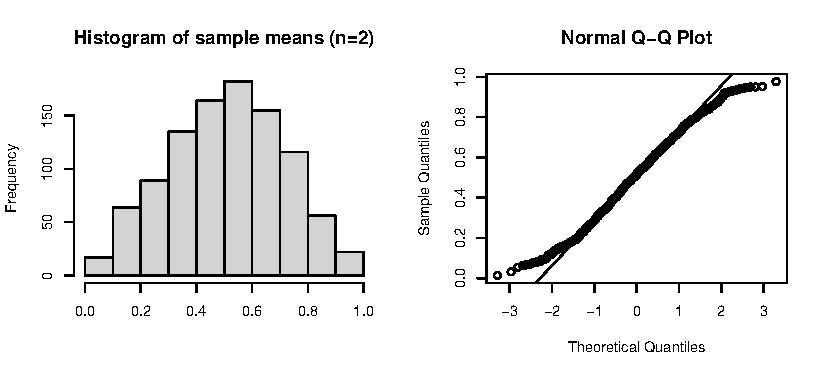
\includegraphics[width=\maxwidth]{figure/unnamed-chunk-2-1} 
\begin{kframe}\begin{alltt}
\hlkwd{mean}\hlstd{(xbars)}
\end{alltt}
\begin{verbatim}
## [1] 0.5104061
\end{verbatim}
\begin{alltt}
\hlkwd{var}\hlstd{(xbars)}
\end{alltt}
\begin{verbatim}
## [1] 0.04123252
\end{verbatim}
\end{kframe}
\end{knitrout}
\bigskip

% {\color{blue}
% \emph{What do you notice?}\\
% 
% The histogram looks bell-curve shaped.  However, the QQ plot has an S-shape, indicating some deviations from the normal distribution (shorter tails, data are less dispersed than a normal distribution).\\
% 
% Also, $\texttt{mean(xbars)} \approx 0.5 = \mu$ and $\texttt{var(xbars)} \approx \frac{1/12}{2} = \frac{\sigma^2}{2}$
% }
\clearpage

\item Use R repeatedly draw 1000 samples of size $n=30$ from $U(0,1)$.  Take the sample mean of the values in each sample.  Make a histogram and normal QQ plot of the 1000 sample means.   Compute the mean and variance of the sample means.  What do you notice?
\begin{knitrout}
\definecolor{shadecolor}{rgb}{0.969, 0.969, 0.969}\color{fgcolor}\begin{kframe}
\begin{alltt}
\hlkwd{set.seed}\hlstd{(}\hlnum{100}\hlstd{)}
\hlstd{xbars} \hlkwb{<-} \hlkwd{rep}\hlstd{(}\hlnum{0}\hlstd{,} \hlnum{1000}\hlstd{)} \hlcom{# initialize vector }
\hlkwa{for}\hlstd{(i} \hlkwa{in} \hlnum{1}\hlopt{:}\hlnum{1000}\hlstd{) \{}
  \hlstd{samp} \hlkwb{<-} \hlkwd{runif}\hlstd{(}\hlnum{30}\hlstd{)}
  \hlstd{xbars[i]} \hlkwb{<-} \hlkwd{mean}\hlstd{(samp)}
\hlstd{\}}

\hlkwd{par}\hlstd{(}\hlkwc{mfrow}\hlstd{=}\hlkwd{c}\hlstd{(}\hlnum{1}\hlstd{,}\hlnum{2}\hlstd{),} \hlkwc{cex}\hlstd{=}\hlnum{0.6}\hlstd{)}
\hlkwd{hist}\hlstd{(xbars,} \hlkwc{main}\hlstd{=}\hlstr{"Histogram of sample means (n=30)"}\hlstd{,} \hlkwc{xlab}\hlstd{=}\hlstr{''}\hlstd{)}
\hlkwd{qqnorm}\hlstd{(xbars)}
\hlkwd{qqline}\hlstd{(xbars)}
\end{alltt}
\end{kframe}
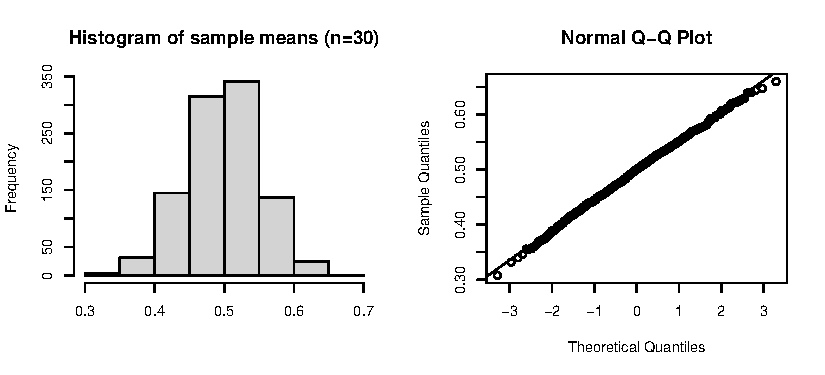
\includegraphics[width=\maxwidth]{figure/unnamed-chunk-3-1} 
\begin{kframe}\begin{alltt}
\hlkwd{mean}\hlstd{(xbars)}
\end{alltt}
\begin{verbatim}
## [1] 0.4985099
\end{verbatim}
\begin{alltt}
\hlkwd{var}\hlstd{(xbars)}
\end{alltt}
\begin{verbatim}
## [1] 0.002890106
\end{verbatim}
\end{kframe}
\end{knitrout}
\bigskip

% {\color{blue}
% \emph{What do you notice?}\\
% 
% The histogram and QQ plot indicate that the sample means are normally distributed when the sample size $n=30$.\\
% 
% Also, $\texttt{mean(xbars)} \approx 0.5 = \mu$ and $\texttt{var(xbars)} \approx \frac{1/12}{30} = \frac{\sigma^2}{30}$
% }
\end{enumerate}



\clearpage

\textbf{The Central Limit Theorem}\\

Let $X_1, X_2, \cdots, X_n$ be a random sample of size $n$ from a population with mean $\mu$ and standard deviation $\sigma$.  Specifically, $X_1, X_2, \cdots, X_n$ are independent and identically distributed (i.i.d.) random variables such that $E(X_i) = \mu$ and $Var(X_i) = \sigma^2$.  Define the sample mean and total as follows:
\begin{align*}
\bar{X} = \frac{1}{n}\sum_{i=1}^n X_i\\
T = \sum_{i=1}^n X_i
\end{align*}

The Central Limit Theorem (CLT) states that when $n$ is large the sample mean $\bar{X}$ is approximately normally distributed with mean $\mu$ and standard deviation $\sigma / \sqrt{n}$.  This is true regardless of the shape of the population distribution for $X$.  To summarize, for large $n$: \begin{align*}
\bar{X} \sim N(\mu, \sigma / \sqrt{n})
\end{align*}
To transform $\bar{X}$ to a standard normal distribution use:
\begin{align*}
Z = \frac{\bar{X} - \mu}{\sigma / \sqrt{n}}
\end{align*}
%mention something about standard error

Similarly, the CLT also states that the sample total $T \sim N(n\mu, \sqrt{n} \sigma)$ for large $n$.\\  
To transform $T$ to a standard normal distribution use: 
\begin{align*}
Z = \frac{T - n\mu}{\sqrt{n} \sigma}\\
\end{align*}  

Remarks:
\begin{itemize}
\item Simulation studies have suggested that $n \geq 30$ is a large enough sample size for the CLT to hold.  However, do not apply this rule blindly.  For highly skewed populations we might need a sample size larger than 30.  For populations that are symmetric, sample sizes smaller than 30 might be sufficient.
\item If the population distribution is normal, then $\bar{X}$ is normally distributed for any sample size $n$.
\end{itemize}

\clearpage

\textbf{Ex1}.  Let $X$ be a random variable with $\mu = 10$ and $\sigma = 4$.  A sample of size $n=100$ is taken from this population. 
\begin{enumerate}[(a)]
\item Find the probability that the sample mean of these 100 observations is less than 9.\\
\vspace{5cm}

% {\color{blue}
% Since $n$ is large $\bar{X} \sim N(\mu, \sigma / \sqrt{n})$ by the CLT.
% \medskip
% 
% So $\bar{X} \sim N(10, 4 / \sqrt{100}) = N(10, 0.4)$
% \begin{align*}
% P(\bar{X} < 9) = P \left( Z < \frac{9 - 10}{0.4} \right) = P(Z < -2.5) = \texttt{pnorm(-2.5)} = \boxed{0.0062}\\
% \end{align*}
% }

\item Find the probability that the sum of these 100 observations is greater than 950.\\
\vspace{5cm}

% {\color{blue}
% Since $n$ is large $T \sim N(n\mu, \sqrt{n} \sigma)$ by the CLT.  
% \medskip
% 
% So $T \sim N(100 \cdot 10, \sqrt{100} \cdot 4) = N(1000, 40)$
% \begin{align*}
% P(T > 950) &= 1 - P(T < 950) = 1 - P\left( Z < \frac{950 - 1000}{40} \right)\\
% &= 1 - P(Z < -1.25) = 1-\texttt{pnorm(-1.25)} = \boxed{0.8943}\\
% \end{align*}
% }
\end{enumerate}

\textbf{Ex2}.  A large freight elevator can transport a maximum of 9800 pounds.  Suppose a load of cargo containing 49 boxes must be transported via the elevator.  Experience has shown that the weight of boxes of this type of cargo follows a distribution with mean $\mu=205$ pounds and standard deviation $\sigma = 15$ pounds.  Based on this information, what is the probability that all 49 boxes can be safely loaded onto the freight elevator and transported.\\

% {\color{blue}
% Let $T = $ the total weight of the 49 boxes.  Since $n$ is large $T \sim N(n\mu, \sqrt{n} \sigma)$ by the CLT.
% \medskip
% 
% So $T \sim N(49 \cdot 205, \sqrt{49} \cdot 15) = N(10045, 105)$  
% \medskip
% 
% Hence, the probability all boxes can be safely loaded is
% \begin{align*}
% P(T < 9800) = P \left( Z < \frac{9800 - 10045}{105} \right) = P(Z < -2.33) = \texttt{pnorm(-2.33)} = \boxed{0.0099}
% \end{align*}
% }
\clearpage
\textbf{Theorem}.  Let $X_1, X_2, \cdots, X_n$ be independent and identically distributed (i.i.d.) random variables.  Let $E(X_i) = \mu$ and $Var(X_i) = \sigma^2$.  Let $\bar{X} = \frac{1}{n} \sum_{i=1}^n X_i$.  Show that $E(\bar{X}) = \mu$ and $Var(\bar{X}) = \sigma^2 / n$.\\

To show this use the following properties of expectation of variance.  Let $X$ and $Y$ be random variables, and $a$ and $b$ constants.
\begin{itemize}
\item $E(aX+b) = aE(X) + b$
\item $Var(aX + b) = a^2 Var(X)$ 
\item $E(X + Y) = E(X) + E(Y)$
\item $Var(X+Y) = Var(X) + Var(Y) + 2Cov(X,Y)$
\item If $X$ and $Y$ are independent then $Cov(X,Y)=0$, and so $Var(X+Y) = Var(X) + Var(Y)$\\
\end{itemize}

% { \color{blue}
% Using these properties:
% \begin{align*}
% E(\bar{X}) = 
% E\left( \frac{1}{n} \sum_{i=1}^n X_i \right) = 
% \frac{1}{n} E \left( \sum_{i=1}^n X_i \right) = 
% \frac{1}{n} \sum_{i=1}^{n} E(X_i)  = 
% \frac{1}{n} \sum_{i=1}^{n} \mu = \frac{n \mu}{\mu} = 
% \mu
% \end{align*}
% 
% \begin{align*}
% Var(\bar{X}) 
% &= Var\left( \frac{1}{n} \sum_{i=1}^n X_i \right) 
% = \frac{1}{n^2} Var\left( \sum_{i=1}^n X_i \right) 
% \stackrel{\text{indep}}{=} \frac{1}{n^2} \sum_{i=1}^{n} Var(X_i)\\ 
% &= \frac{1}{n^2} \sum_{i=1}^{n} \sigma^2 
% = \frac{n \sigma^2}{n^2} 
% = \frac{\sigma^2}{n}
% \end{align*}
% }

%Induction can be used to more formally show that the expectation of the sum of RVs is the sum of the expecations of RVs in (1).  For instance, let $X$, $Y$, and $Z$ be RVs and $W = Y+Z$ then $E(X+Y+Z) = E(X + W) = E(X) + E(W) = E(X) + E(Y+Z) = E(X) + E(Y) + E(Z)$. 
 



\end{document}
